\chapter{Experiments}
\label{ch:Experiments}

In this chapter, we will compare the runtimes of three summation procedures:
\begin{itemize}
  \item the binary tree summation algorithm as presented in chapters \ref{ch:BinaryTreeSummation} and \ref{ch:Implementation}
  \item the ReproBLAS reduce operation
  \item a bitwise-irreproducible implementation with \texttt{MPI\_Allreduce} and \texttt{std::accumulate} as baseline.
\end{itemize}

\section{Experimental Setup}
\label{sec:ExperimentalSetup}
The machine \textit{i10pc138}, which has two AMD EPYC 7713 CPUs with $64$ cores each, $2$ threads per core for a total of $256$ CPUs and $1024$ GB of DDR4 main memory, executed all benchmarks with less than $257$ \glspl{pe}.
The bwUniCluster 2.0 ran all other benchmarks.

\begin{table}
\centering
\begin{tabular}{r|l}
\textbf{dataset name} & \textbf{number of summands} \\
354 & $460$ \\
multi100 & $767$ \\
prim & $898$ \\
fusob & $1\,602$ \\
dna\_rokasD4 & $239\,763$ \\
aa\_rokasA8 & $504\,850$ \\
dna\_rokasD1 & $1\,327\,505$ \\
aa\_rokasA4 & $1\,806\,035$ \\
dna\_PeteD8 & $3\,011\,099$ \\
dna\_rokasD7 & $21\,¸410\,970$ \\
\end{tabular}
\caption{Overview of benchmark datasets}
\label{table:datasets}
\end{table}

Input data was extracted from RAxML-NG workloads in the form of an array of double-precision floating point numbers representing per-site log-likelihood values.
The datasets come in various sizes, depending on the multiple sequence alignment length. Table \ref{table:datasets} gives an overview.
Each benchmark run performs the following steps for each summation mode (\texttt{reproblas}, \texttt{allreduce}, \texttt{tree}) and each dataset:
\begin{enumerate}
\item Load input data from file and distribute it among the \glspl{pe}
\item Perform the summation $100$ times, measuring the duration for each time
\item Prune the first and last eight measurements
\end{enumerate}

\section{Results}
\label{sec:Results}

\begin{figure}
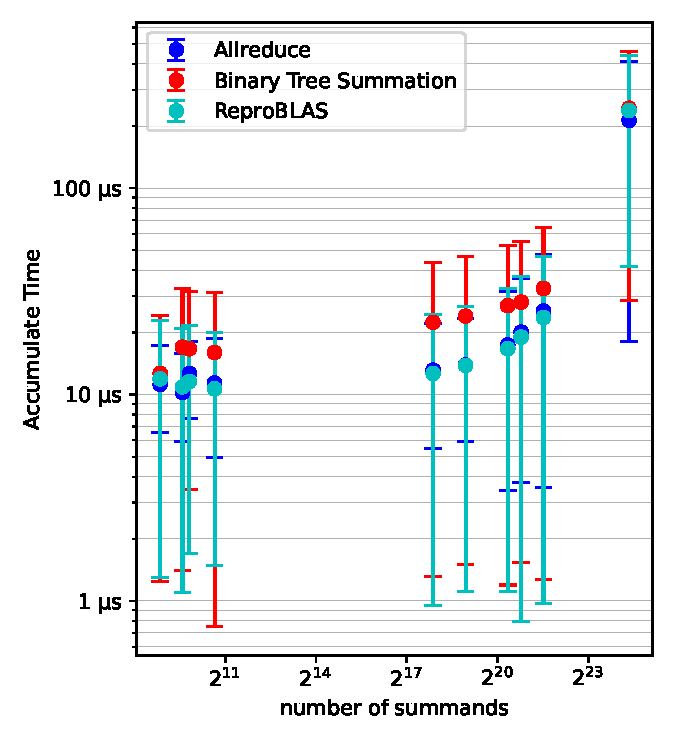
\includegraphics[scale=1]{figures/benchmarkScatter.pdf}
\caption{Summation runtime for different datasets across $256$ \glspl{pe}}
\label{fig:benchmarkOverview}
\end{figure}

Figure \ref{fig:benchmarkOverview} shows the runtime measurements across all datasets as scatter plot.
Error bars depict the standard deviation of measurements.



\section{Verification of Reproducibility}
\label{sec:VerificationOfReproducibility}

\section{Scaling Behaviour}
\label{sec:ScalingBehaviour}